\documentclass[12pt]{article}
\usepackage{graphicx}
\usepackage{url}
\usepackage[authoryear,round]{natbib}


\title{Outline flowCore paper}

\author{Florian Hahne*\\
  Nolwenn LeMeur*\\
  Byron Ellis\\
  Ryan Brinkman\\
  Perry Haaland\\
  Errol Strain\\
  Deepayan Sarkar\\
  Josef Spidlen\\
  Robert Gentleman
 }

\begin{document}

\vspace{2ex} 

The paper will deal with the capabilities offered by flowCore for
handling flow cytometry data in R. The main focus should be on
high-throughput and how our infrastructure can be used to deal with
such data. We don't want to write a user manual but rather highlight
the problems that arise from high throughput flow applications and the
solutions we offer. A strong point should be on integration of our
infrastructure in the flow world. flowCore is intended to be a
development platform for other scientists, we don't want to provide
full-fledged solutions but rather tools for others to devise such
solutions.

It would be nice to show these things on one data set in the form of a
use case, but that is open to discussion. The problem with such an
approach is that it often looks like a software manual which is not
what we should be aiming for. 

\bigskip
The author list is also still up for discussion, listed here are all
the names that came up during the last telephone conference. NLM and
FH are supposed to share first authorship.

\bigskip
Target journal should be Cytometry, and there are two flavors:
Cytometry A deals with more general topics while Cytometry B is more
geared towards clinical applications. Florian suggests Cytometry A,
here is a link to the author instructions:
\url{http://www3.interscience.wiley.com/journal/33945/home/ForAuthors.html}.
They require the standard Materials and Methods, Results and
Discussion structure which might not be suited for our needs. FH
hasn't found out about alternative methods-type articles yet.  

{\bf NLM:} We can suggest to the editor new format for software/methods
oriented paper?

{\bf RB:} I know the editor and would be happy to speak to him
regarding methods-type articles or other issues if needed.

Also it is not clear from their web page whether they support LaTeX
manuscript submissions but FH would strongly argue for using
LaTeX. They do accept pdf submission.

{\bf RB:} Cytometry does not accept LaTeX (we've tried). While they say
they will accept PDF they made us convert PDF to Word in the past. I
was able to do this reasonably well with a third-party software tool.

\bigskip
There is an svn repository set up at
\url{https://hedgehog.fhcrc.org/gentleman/bioconductor/trunk/madman/Rpacks/flowCore/paper}
which is also the repository for the flowCore source code. All
contributors should already have usernames and passwords, if not
please contact FH.

\bigskip
There have been discussions on how much technical detail we want to
provide and how and where example should be given:

{\bf PH:} Do we have a simple illustration of why we need to be able to
program with flow data in order to do more meaningful science? Could
we say something about finding populations or automated gating as
being enabled by flowCore?  We have found the lattice plots and the
ability to make overlays very helpful. Could we include an example
where these capabilities would be helpful?

{\bf RB:} Enabling automated gating is certainly true as we have just had a
manuscript accepted for automated gating that relies on flowCore.

{\bf PH:} It seems to me some examples of what flowCore makes possible needs
to be at the heart of the paper. That doesn't mean that we need to
show a detailed analysis.

{\bf ES:} I also think that use cases/examples are very important for selling
the software.  I don't believe we need a complete analysis vignette in
the paper, but specific examples that I've found useful include
\begin{itemize}
\item Correcting for the effects of cell size on autofluoresence using
  Florian's regression,
\item Automating report generation (using Sweave), including making
  overlay plots (supposed hard to batch this job in FlowJo?),
\item automated gating,
\item population finding (using mclust, other R density tools, etc).
\end{itemize}

{\bf RB:} The code examples in the supplementary material, but could
be highlighted in the main text with the pretty results (the selling
point to biologists), something like: “For example, with a short
section of user-configurable code (see Supplementary Material) it is
possible to automate the processing of 1000s of individual FCS data
files and generate high quality reports (Figures 1, 2) including such
steps as quality checking plots, correcting for cell size on auto
fluorescence, followed by automated gating.  This code can be freely
extended and modified by users as the underlying code is all available
at no cost under an open source license ”.  I think it’s important
to remember the audience. The people reading Cytometry we need to
convince on the importance of flowCore are the biologists, and putting
code examples in the main text won’t help, and will likely
hinder. The programmers/statisticians/bioinformaticians out there will
go to the code in the Supplementary Material/Vignettes section
already. All the biologists need to see are the pretty pictures that
let them interpret their data. Highlighting the support network
available (Bioconductor list) will be important in terms of hand
holding.  In terms of making biologists happy, it might be worth
talking to Adam about plans to call R from FlowJo. At the least it
should be highlighted that this is possible in the generic sense.

{\bf PH:} agree that the code examples should go in the supplemental
materials, and I like the examples that Ryan gives below. One thing
that we have found to be very challenging to the biologists is that
they no longer do the primary analysis of their data. We have
addressed that by highlighting the ability to programmatically analyze
lots of data, most of which has fairly straightforward results and
then to focus the biologists attention only on the data that needs
expert interpretation/tweaking.

{\bf BE:} This is, unfortunately, somewhat of a problem---the biologist (as
a community, I realize that there are specific individuals to whom
this does not apply and that I'm likely especially sensitive to this
phenomenon) doesn't believe that data can be analyzed apart from
direct inspection. It might be worth stressing that flow* allows for
not only automated analysis, but provides a platform for improving
collaboration. Actually, it occurs to me that this is probably "the
important bit" for the data structures, which are not particularly
profound in and of themselves---they mostly take the form they do
because that's the way Bioconductor does things in general. However,
what they buy you is a standard mechanism for the organization of
annotation of experiments that is suitable for programmatic
manipulation rather than the usual ad hoc collection of 30 randomly
formatted Excel spreadsheets that may or may not have anything to do
with the actual flow data you have.

{\bf PH:} I agree with that. We need to explain to the biologists that they
"can't get there from here" unless they adopt better data organization
and automated analysis and work collaboratively. It would be nice to
think about how we would make that argument.

\bigskip











\maketitle

\section*{Introduction}

Traditionally, flow cytometry (FCM) has been a tube-based technique
limited to small-scale laboratory and clinical studies.  High
throughput methods for flow cytometry (FC-HCS) have recently been
developed and are now used in both basic and clinical research. Today,
the need for flexible and well structured computational tools to
efficiently handle and analyze FC-HCS has increased
considerably. Indeed, the amount of information generated by these
technologies must be stored, managed, and needs to be summarized in
order to be accessible to the researcher. However, the absence of any
shared research platform, which bioinformaticians, computer scientists,
and statisticians can utilize to develop novel or standard methods for
flow cytometric analysis has become problematic. We believe that the open
source statistical software R in conjunction with the Bioconductor
Project can fill this gap.  In this paper, we propose R data
structures to handle flow cytometry data through the main steps of
importing, storing, assessing and preprocessing data from FC-HCS
experiments. These structures, along with a range of specialized
methods for compensation, transformation, gating and additional
preprocessing steps, are implemented in the newly developed
Bioconductor package flowCore.  We envision flowCore to be a solid
foundation for researchers to efficiently handle FC-HCS data and for
future development of new methods and tools for their coherent
analysis.


\subsection*{R and Bioconductor}
R is a solid statistical programing environment, particularly geared
towards the analysis of large numeric datasets typical to arise from
high throughput experiments such as microarray gene expression
analysis or FC-HCS. Today, the R open source project offers a wide
range of statistical and visualization methods developed for various
fields of application. In addition, R is a research platform which
bioinformaticians, computer scientists, and statisticians routinely
use to develop novel tools and methodology for statistical data
analysis. For biological applications, the Bioconductor project has
become the standard toolset \citep{gentleman2006bos} to process data
spanning a diversity of research fields from genomics to proteomics to
complex cell biology. This shared platform proved to be particularly
beneficial for the development of analysis routines for microarray
gene expression data, and by today many of these early innovations
have been incorporated into commercial software products, thus greatly
improving the quality of gene expression data analysis. In this
context, shared data structures have been shown to be essential for
such a collaborative effort.


\subsection*{Existing data standards and conventions}
Currently, data from flow cytometry experiments are stored in single
files following a well-defined data standard (FCS). This standard
attempts to capture as much of the accompanying meta information as
possible, most of which is produced by the measurement instrument or
has to be supplied manually by the operator upon experiment
setup. However, the recent developments in high-throughput flow
cytometry are shifting the focus of interest away from single-tube
based measurements towards large and complex experimental designs with
dozens of co-variates and influencing factors. Self-contained and
self-reflective data structures are a prerequisite to allow for
coordinated analysis of such experiments. Most of the currently
available software solutions offer only limited support for such
structures, or make use of containers like XML or binary storage
formats that are designed specifically for the mostly GUI-driven user
interfaces and hence are not easily amenable to programmatical
access. In addition, the closed-source nature of most of these
products makes it virtually impossible to connect and integrated the
data.

Traditionally, the majority of flow cytometry experiments have been
analysed manually by direct data inspection in one ore tow dimensions,
or by very basic comparisons of summary statistics. We believe that
these approaches do not give justice to the highly complex nature of
FCM data, in particualar, they discard many of the fundamental aspects
such as underlying distribution of the data or the
high-dimensionality. In addition, the subjective character of manual
analyses are a major obstacle for reproducibility. For FC-HCS data,
unassisted manual inspection is no longer feasible, and robust
statistical methods need to be developed to point the investigator to
the interesting aspects of the data or to potential problems. While
the expert knowledge of immunologists and researchers remains crucial
for the understanding of FCM data, we believe that tight collaboration
with other research fields such as statistics and computer science can
greatly improve the relevance of flow cytometry in today's
high-throughput biological sciences.

These issues are currently being addressed by emerging new flow
cytometry data standards developed in collaboration with the ISAC Data
Standards Task Force.  The Gating-ML Candidate Recommendation (CR)
represents a proposal on how to form unambiguous XML-based gate
definitions, which can facilitate the interchange and validation of
data between different software packages with the potential of
significant increase of hardware and software interoperability. Gates
may be ordered into a hierarchical structure to describe a gating
strategy. They may be applied on parameters as in FCS files or on
transformed parameters as described by an explicit parameter
transformation. This allows to encode a simple analytical work flow,
which is sufficient in order to reconstruct the analysis
programmatically. 

The flowCore framework presented here offers import functionality for
raw data FCS files along with their complete set of file-specific meta
information (Figure~\ref{fig1:FrameWork}).  Moreover, it is one of the
very first software implementations of the Gating-ML CR, which opens
the possibility to integrate flowCore in existing work flows and to
communicate with virtually every other FCM tool that adheres to the
proposed standard. In addition, the software is platform independent,
running on various operating systems including Windows, Mac OS X and
Linux/Unix.

flowCore is not a GUI-driven software, and all operations are
currently done using a command line interface. Conceptually, it is
possible to add a more elaborate user interface on top of that,
however we strongly focus on programmatic access to enable the
convenient development of novel analysis methods. By taking the burden
of data management from the programmer and by providing well-defined
APIs and a structured class hierarchy, it is possible to readily test
new ideas and to easily extend the frameworks functionality. Both the
underlying R and Bioconductor software and flowCore itself are open
source and open development projects, thus community involvement in the
developing process is highly appreciated.



\section*{Basic data structures}
\subsection*{flowFrame}
flowCore's primary task is the representation and basic manipulation
of flow cytometry data. This is accomplished through a data model very
close to that adopted by other Bioconductor packages used for gene
expression analysis, and thus familiar to most Bioconductor
users. Similar to any other flow tool, the basic unit of organization
in flowCore is a collection of events. We call the structure that hold
this data a flowFrame. All relevant information for the collection are
stored along with the matrix of raw data values and can be accessed
programmatically. Most prominently, these are descriptors of the
stains used in the experiment and the respective measurement channels,
information about compensation performed at the instrument side and
any additional keywords the user deems to be important to annotate the
data. A number of quality checks are performed during the creation of
a flowFrame to ensure data integrity. There is an extended interface
that allows for the standardized interaction with the flow data, thus
enabling the development of more specialized tools for specific tasks
of the data analysis process.

\subsection*{flowSet}
In high-throughput flow cytometry, many of the analysis tasks need to
be performed consistently across multiple flow measurements, hence we
introduce the concept of a collection of flowFrames called a
flowSet. flowSets store the relevant information associated with each
individual frame such as descriptions of the samples or the treatment
to which a sample was subjected, and they manage the consistent
application of operations on the individual flowFrames. The burden of
keeping score of the annotation is shifted from the user to the
infrastructure, thus reducing the risk of mixups and errors that are
all too common when dealing with complex data in the ususal way:
namely, more or less ad hoc spreadsheets that lack a controlled
structure. In general, there is no native ordering to a flowSet, which
in a way reflects the still predominant application of tube-based
experiments rather than experiments following a plate-design. However,
the flowSet structure can be readily extended to also accommodate such
spatial information [citing plateCore - Any reference here Perry, Errol?]

%%Figure1 Diagram of the data structures and the basic operations
\begin{figure}
\centering
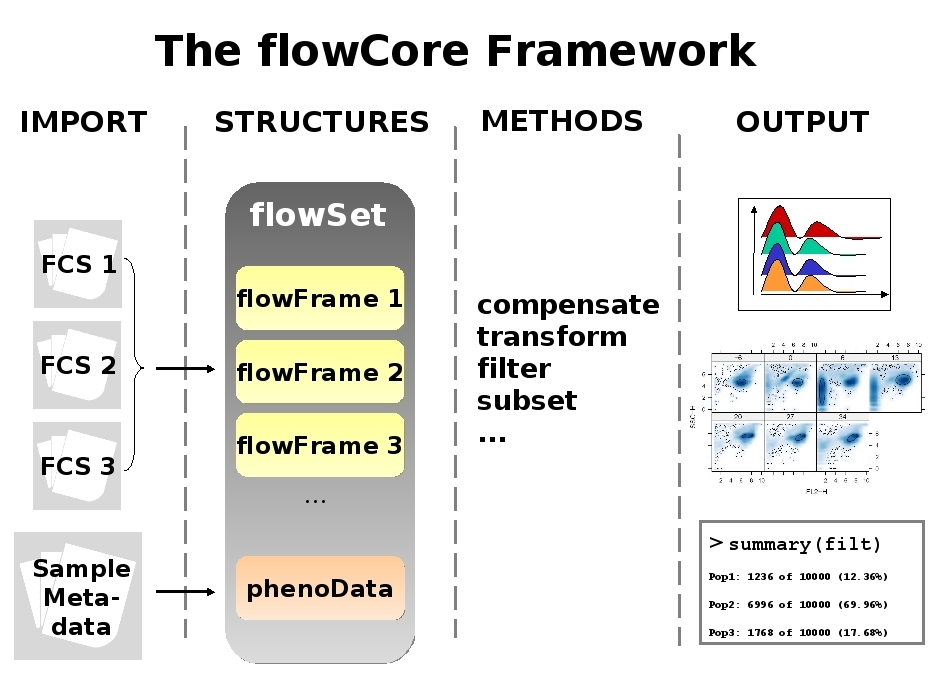
\includegraphics[width=0.9\textwidth]{Figure1-flowCoreFrameWork.jpg}
\caption{\label{fig1:FrameWork}{The flowCore frame work.For each experiement,
  FCS files, phenotypic and meta data can be store in a flowSet. Each
  flowFrame of a flowSet corresponds to one FCS file.  Any basic
  operation (compensate, filter, ...) can be applied on a flowSet or a
  flowFrame.Different summary output can be generated with flowCore or
  the associated packages.}}
\end{figure}


\section*{Standard flow operations}
The basic operations in flow cytometry analysis are almost always the
same: the data need to be compensated (if not already done on the
instrument side), often transformed and sup-population of interest
need to be selected based on a set of (predominantly sequential)
gates. All software solutions for flow data analysis offer more or
less elaborate support for these kinds of operation, most of them in
an interactive, GUI-driven spirit. The approach we have taken in
flowCore is to abstractly describe these operations and build a set of
tools to perform them on both flowFrames as well as on entire
flowSets. While transformation and to a certain extent also
compensation are fairly routine operations with only limited potential
for improvement, being able to implement new methodology for gating of
flow cytometry data and extending the capabilities of flowCore through
the usual ways of object oriented programming is a feature, that
clearly sets our framework apart from all the other flow toolsets
around. By factoring out as much of the bookkeeping as possible,
programmers can focus on the actual operations rather then having to
deal with the tedious details of data integration and access. Third
party methods implemented by others can act on their own as
first-class citizens in the analysis framework, without breaking the
workflow or the basic infrastructure. This design allows for the
straight forward extension of flowCore's capabilities and already
fostered the development of a number of valuable
improvements \citep{lo2008agf, sarkar2008ufv}.




\subsection*{Transformation and compensation}
Proper transformation have been proven beneficial for both data
visualization and modelling \citep{lo2008agf}. All the
major transformations that are routinely used in flow cytometry
analysis have been implemented in flowCore. Furthermore, the design of
the R language makes it easy to define arbitrary functions to apply to
the data of individual flowFrames or entrire flowSets,
respectively. Compensation is available for both flowFrames and
flowSets, and the software also offers functionality to compute
spillover or compensation matrices from a set of appropriate
compensation samples. 



\subsection*{Gating}
In flowCore, gates are represented as individual classes that can be
extended in an object oriented manner. All basic gate types such as
rectangular gates, ellipses and polygon gates are implemented as part
of the base framework. In addition, we introduce the notion of
data-driven gates, or filters, for which the necessary parameters are
computed based on the properties of the underlying data, for instance
by modelling underlying data distribution or by density
estimation. The ability to programmatically access gates is a
prerequisite for automated or semi-automated gating. By utilizing a
unified interface for all different types of gates, the user is able
to subset data sets as well as to create summary statistics, like the
proportions of events falling in single gates or in the combinations
of multiple gates. Conmplex combinations and hierarchies of gates can
be captured in objects of class filterSet, allowing to apply
multi-step gating strategies. The definition of gates in flowCore
follows the Gating-ML CR, thus any flowCore gating strategy can be
reproduced by any other software that also adheres to the standard.

\section*{Related flow packages}
In addition to the flowCore package that offers basic infrastructure,
we have implemented a range of additional Bioconductor packages that
are dedicated to more specific tasks of flow cytometry data analysis
(Figure~\ref{fig2:flowWheel}). The flowViz package provides
sophisticated data visualization tools, that make use of multivariate
trellis plotting. These functions can be used to quickly generate
customized plots for extended cytometry data sets for both direct data
inspection and quality control. The flowQ package offers more advanced
quality assurance (QA) methodology and a framework to create
interactive web-based reports of QA results. Most of flowUtil's
content deals with data import and output from and to flowCore and the
flow-cytometry specific standard markup languages. Finally, flowStats
provides statistical methods that are relevant in the context of flow
cytometry data analysis.

\begin{figure}
\centering
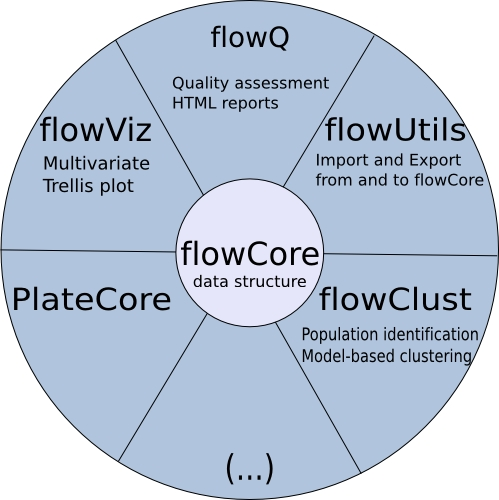
\includegraphics[width=0.6\textwidth]{Figure2-flowWheel-version4.jpg}
\caption{\label{fig2:flowWheel}{The flowCore Suite: visualization and analysis
  packages relying on the flowCore data structure.  Dedicated packages
  have been developped using the flowCore data structure for
  manipulating the experiemental data: flowViz is a data visualization
  package; flowQ helps at data quality assessment; flowUtils provides
  xml parser, flowClust proposes population 
  filtration using model-based clustering}}
\end{figure}

\section*{Application}
The flowCore package has already been applied in the analysis of a
number of datasets \citep{gasparetto2004ice,brinkman2007hcf}, and
several other Bioconductor packages are making use of its code
base. As an example, \cite{lo2008agf} have recently proposed an
automatic gating approach via robust model-based clustering using the
flowCore data model and infrastructure (implemented in the
Bioconductor package flowClust). Another package providing more
specialized support for experiments conducted on microtitre plates is
currently being developed. The documentation of all of flowCore's
features is way beyond the scope of this publication. Instead, we
want to use a single example to demonstrate some of the software's
hallmarks, that is, the concept of data-driven automated gating, the
integration of existing software into the framework and the generation
of publication-quality graphics for data visualization. The data used
for this example are flow measurements of human T-lymphocytes from 30
different patients, stained for both the CD4 and CD8 markers.

A very basic matrix of scatterplots is shown in Figure \ref{xyplot},
where each panel in the matrix represents the data of one individual
patient. Instead of plotting individual points, the local bivariate
density of the data is shown as a false color image. For each panel,
the outlines of the regions identified in the automated gating
operation described below are added to the plot. The input to the
plotting function is either a single flow frame or a complete flow set
object, and all available metadata can be accessed to control the
appearance and the composition of the plot. Similarily, gate objects
are directly passed on to the plotting function and are included in
the plot if possible. Besides the very basic scatterplot shown here,
there is a wealth of additional data visualizations available in the
flowViz package \citep{sarkar2008ufv}, all making use of flowCore's data
models allowing to easily arrange the data according to numerous
experimental factors. Furthermore, the design and the API of the
visualization software itself is very generic, and the user can
readily extend its capabilities by providing self-defined plotting
functions.

Static gating for all samples in a high-throughput flow cytometry
experiment is often not an option, since the measured variables tend
to vary between different treatments or over time. Automated or
data-driven gating tries to estimate the gating regions from the
underlying data, thus providing a fast objective solution to the
analysis of potentially very large and diverse data sets
\citep{lo2008agf}. One of the automated gating methods implemented in
flowCore is based on identifying areas of significant curvature in a
kernel density estimate of the data
\citep{wand2008,wand2008_2}. Assuming that the regions of interest are
of high density, the software is able to reliably detect them in
either the one ore the two-dimensional density landscape. Kernel
density estimation is a well-known problem in statistical computing,
and a lot of effort has been invested in the development of good
software to address it \citep{wand2008,wand2008_2}. The modular design
of R, Bioconductor and flowCore allows to easily integrate these
existing solutions into our framework. Instead of re-writing existing
code, we are able to include it via the well tested distribution
mechanism provided by R's software package system. This process is
bi-directional, and all funtionality implemented in flowCore is
available to other package authors, as we have seen with the
afore-mentioned flowClust package.

In developing flowCore, we tried to provided a unified develoment and
analysis platform for flow-cytometry data. The scope and complexity of
the technology is evolving rapidly, and a collaborative effort in
devising new methodolgy has been proven beneficial for a number of
different biological and computational biology challenges. We hope
that our framework will be the foundation for fruitful shared research
by many calloborators from multiple scientific fields, further pushing
the boundaries of the exiting and still promising flow
cytometry technology.



\bibliographystyle{plainnat}  
\bibliography{flowCoreRef} 
\end{document}

